\documentclass{jarticle}
\usepackage[dvipdfmx]{graphicx}
\usepackage{listings,jlisting,url,here}

\lstset{%
  language={C},
  basicstyle={\small},%
  identifierstyle={\small},%
  commentstyle={\small\itshape},%
  keywordstyle={\small\bfseries},%
  ndkeywordstyle={\small},%
  stringstyle={\small\ttfamily},
  frame={tb},
  breaklines=true,
  columns=[l]{fullflexible},%
  numbers=left,%
  xrightmargin=0zw,%
  xleftmargin=3zw,%
  numberstyle={\scriptsize},% stepnumber=1,
  numbersep=1zw,%
  lineskip=-0.5ex%
}


\title{グループレポート}
\author{6119019092 織田武瑠 6119019207 矢野大暉 6119019056 山口力也}
\date{2019/11/22 提出}

\begin{document}
\maketitle

\section{開発期間11/18~11/24の進捗状況} 

\subsection{進展事項}
今回の開発期間では,ゲームの設計として主に
\begin{itemize}
\item プレイヤーの移動の不具合を改善するための方法を検討
\item ネットワーク通信をしている状態で金塊をとれるよう実装
\item スタート画面の実装
\item プログラムの統合と,ヘッダファイル等の整理
\item 敵の移動の実装
\item 参照バグの修正
\end{itemize}
を行った.以下にその詳細を示す.

\subsection{プレイヤーの移動の不具合を改善するための方法を検討}
プレイヤーに斜め移動をさせる際,上下左右の移動に比べて速度が早くなるため,その対策の検討をした.
実装方法としてプレイヤーの座標を実数で保存しておき,斜め移動の際に$\frac{1}{\sqrt2}$を掛けることによって斜め移動を実現できる可能性があることがわかった.

\subsection{ネットワーク通信をしている状態で金塊をとれるよう実装}
金塊を取る処理をネットワーク通信下でもできるように実装した.

\subsection{スタート画面の実装}
ゲーム起動時に,スタート画面が表示されるように実装した.
ゲーム開始と,ゲーム終了の2つ選択できるボタンを実装しており,決定ボタンを押すことでそれぞれの処理を行う.
実装した画面を図\ref{fig:start}に示す.

\begin{figure}[H]
\begin{center}
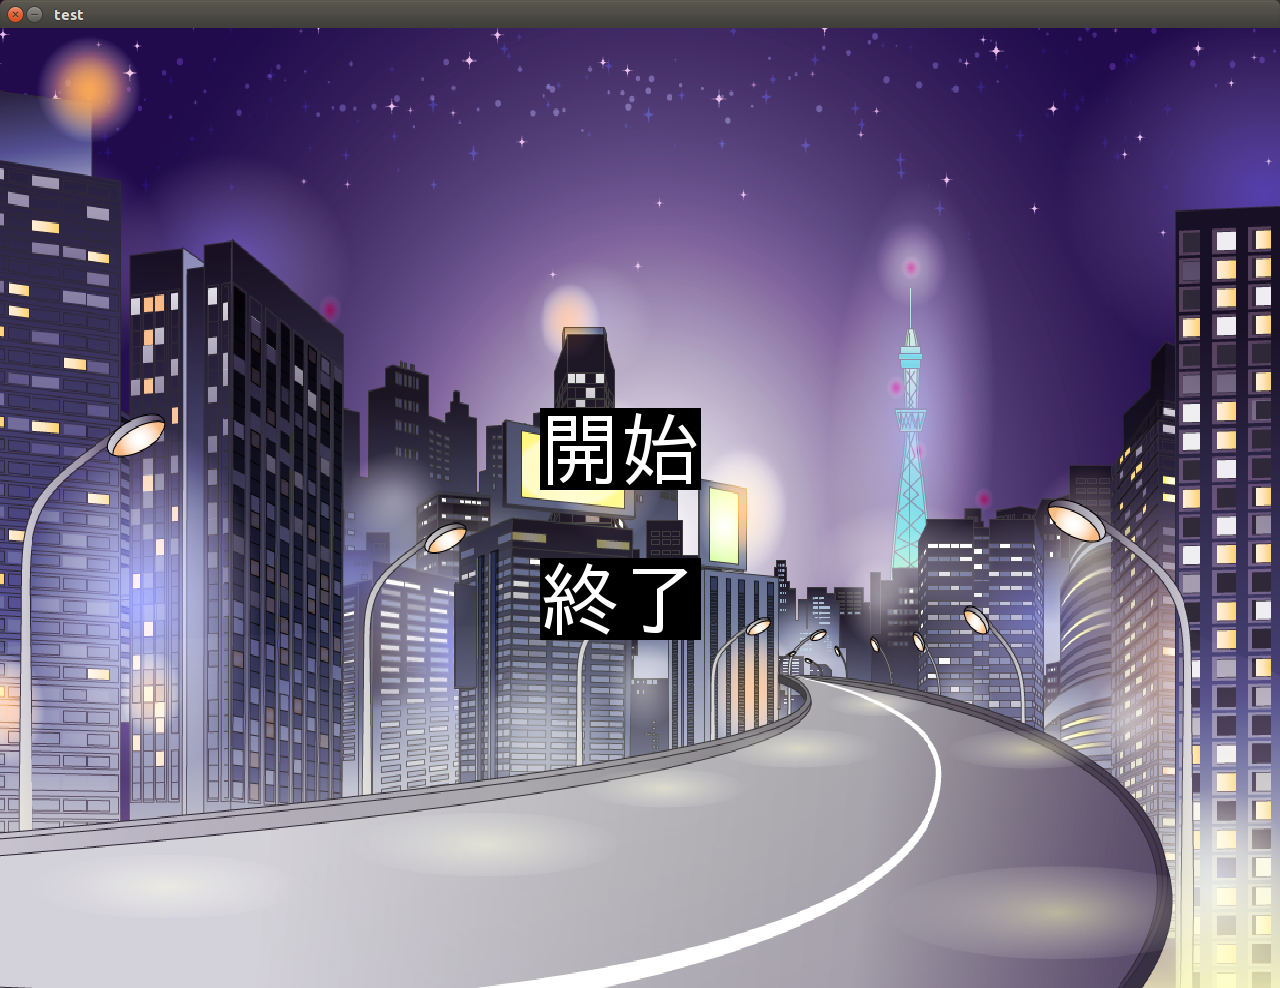
\includegraphics[width=\linewidth]{./zu/gamestart.png}
\caption{スタート画面(仮)}
\label{fig:start}
\end{center}
\end{figure}

\subsection{プログラムの統合と,ヘッダファイル等の整理}
スタート画面を表示する機能のプログラムを統合した.
その際,ヘッダファイルの対応関係を見直し修正した.

\subsection{敵の移動の実装}
敵の移動方向をマップの位置ごとに変える機能を実装した.

\subsection{参照バグの修正}
プレイヤーの情報がカメラに入ってしまい,カメラの表示位置がおかしくなるというバグが発生した.
マップ作成機能において,必要なエラー処理が抜けていたためミスに気づくのに時間がかかったが,修正した.

\end{document}
